\documentclass[10pt]{exam}
\usepackage[hon]{template-for-exam}
\usepackage{enumitem}
\usepackage{tikz}
\usepackage{multicol,graphicx}
\usetikzlibrary{shadings,decorations.pathmorphing,arrows.meta}



\def\mytitle{Chapter 5 (Circular Motion)}
\author{Rohrbach}
\date{\today}

\def\mymaketitle{
  \begin{flushleft}
    {\LARGE \textbf \mytitle \par}
  \end{flushleft}
}



\begin{document}


\mymaketitle



\newcommand{\stampbox}[1]{

  \hfill
  \begin{tikzpicture}[every text node part/.style={align=center}]
     \node[gray!50,draw,rounded corners] at (0,0) 
      {\sc Stamp \\ \sc Here \\ \small #1 \sc Points};
  \end{tikzpicture}
  \vspace{1em}
  
  \hrule

}

\begin{center}

  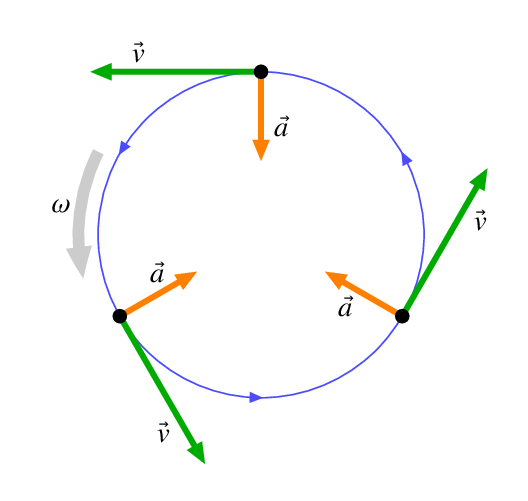
\includegraphics[scale=0.3]{circ.png} \hspace{10em}
  %
  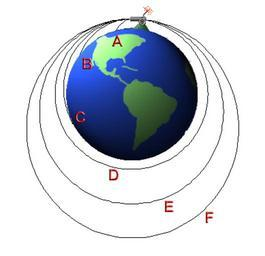
\includegraphics[scale=0.6]{orbitingcannonballs.jpg}
\end{center}

\section*{Homework Check A (collected Mon, Nov 18)}


%%%%%%%%%%%


\paragraph{Basic Circular Motion} p. 132 \#1, 2, 4, 5, 69
\dotfill Complete by Thu, Nov 14

\stampbox{5}


%%%%%%%%%%%


\paragraph{Multi-Force/Friction} pp. 132-133 \#7, 8, 15, 19, 73
\dotfill Complete by Mon, Nov 18

\hfill \textbf{\emph{Homework Quiz}}

\stampbox{5}


%%%%%%%%%%%






\subsection*{Answers}

\begin{multicols}{3}

  \begin{itemize}[noitemsep]
    \item[1. ](a) 1.01 m/s$^2$; (b) 22.7 N
    \item[2. ] 5.4 $g$'s
    \item[4. ] 3.9 m/s$^2$
    \item[5. ] 13.3 m/s
    \item[69.] 28.3 m/s
    \item[7. ] 33.6 m/s
    \item[8. ] 0.57
    \item[15.] 0.21
    \item[19.] (a) 5965 N; \\ (b) 379.3 N; \\ (c) 29.4 m/s
    \item[73.] 9.1 m/s
    
    
    
  \end{itemize}
  
\end{multicols}

\noindent
{\footnotesize Homework will be accepted for full credit until the test.
Homework turned in after the test will be accepted for half credit
until the Unit 3 Test.
\emph{Please remember that you will not be eligible to complete 
test corrections if you do not turn in your homework.}}

\vspace{1em}
\hrule 


%%%%%%%%%%%%%
%%%%%%%%%%%%%

\pagebreak

\mymaketitle

\section*{Homework Check B (collected on Test Day)}

\paragraph{Universal Gravitation} pp. 133-134 \#28, 29, 32, 33, 35, 39
\dotfill Complete by Fri, Nov 24

{\sc See reference page for a list of planetary masses/radii}

\stampbox{5}


%%%%%%%%%%%


\paragraph{Satellites} p. 134 \#46, 52, 80
\dotfill Complete by Fri, Nov 24

{\sc See reference page for a list of planetary masses/radii}

\stampbox{5}


%%%%%%%%%%%

\paragraph{Conceptual Questions} pp. 130-131 \#2, 3, 5, 8, 10, 11, 20
\dotfill Complete by Fri, Nov 24
   
{\sc These questions should have at least one full sentence 
      of explanation}

\stampbox{5}

%%%%%%%%%%%%%%

\paragraph{Misconceptual Questions} pp. 130-131 \#1-10, 12
\dotfill Complete by Fri, Nov 24
   
{\sc You do not need to get this one stamped,
but these are good review for your test!}

\vspace{1em}
\hrule

%%%%%%%%%%%%%%

\paragraph{Bonus Problems!} p. 132 \#10; p. 133 \#30; p. 135 \#67
\dotfill Turn in separately on test day!

\vspace{1em}
\hrule


%%%%%%%%%%%%%%

\paragraph{Test} Half the test will be on Mon, Nov 25; the other half will be on Tue, Nov 26.

\vspace{1em}

\hrule

\subsection*{Problem Answers}

\begin{multicols}{3}

  \begin{itemize}[noitemsep]
    \item[28.] 2014 N
    \item[29.] Earth: 24 kg, 235.2 N; \\ Planet: 24 kg, 288 N
    \item[32.] 2.45 m/s$^2$
    \item[33.] 1.62 m/s$^2$
    \item[35.] \SI{6.5e23}{\kilo\gram}
    \item[39.] (a) 9.78 m/s$^2$;  (b) 2.44 m/s$^2$
    \item[46.] 5,973 m/s
    \item[52.] 1.41 hr
    \item[80.] 1.97 hr
    
  \end{itemize}
  
\end{multicols}

\subsection*{Misconceptual Answers}

\begin{multicols}{7}

  \begin{itemize}[noitemsep]
    \item[1. ] b
    \item[2. ] e
    \item[3. ] c
    \item[4. ] d
    \item[5. ] b
    \item[6. ] a
    \item[7. ] d
    \item[8. ] f
    \item[9. ] c
    \item[10.] b
    \item[12.] d
  
  \end{itemize}
  
\end{multicols}

\pagebreak



%%%%%%%%%%%%%%
%%%%%%%%%%%%%%
%%%%%%%%%%%%%%


\section*{Reference Sheet}

\subsection*{New Equations}

\begin{align*}
  a_C        &= \frac{v^2}{r} &
  \Sigma F_C &= ma_C = \frac{mv^2}{r}  &
  v          &= \frac{2\pi r}{T} &
  F_G        &= \frac{Gm_1 m_2}{r^2} \\
  &&&&&& G   &= \SI{6.67e-11}
                {\newton\meter^2\per\kilo\gram^2}
\end{align*}


\subsection*{Old Equations}

\begin{align*}
  \Sigma F &= ma &
  F_G      &= mg &
  F_f      &= \mu F_N
\end{align*}


\subsection*{Other Useful Data}

\begin{center}
  \begin{tabular}{lll}
    \hline
    Earth: & Mass           & \SI{5.98e24}{\kilo\gram} \\
           & Radius (mean)  & \SI{6.38e3}{\kilo\meter} \\
    Moon:  & Mass           & \SI{7.35e22}{\kilo\gram} \\
           & Radius (mean)  & \SI{1.74e3}{\kilo\meter} \\
    Sun:   & Mass           & \SI{1.99e30}{\kilo\gram} \\
           & Radius (mean)  & \SI{6.96e5}{\kilo\meter} \\ \hline
    \multicolumn{2}{l}{Earth-Sun Distance (mean)} & 
                              \SI{1.496e8}{\kilo\meter} \\
    \multicolumn{2}{l}{Earth-Moon Distance (mean)} & 
                              \SI{3.84e5}{\kilo\meter} \\
                              \hline\hline
  \end{tabular}
\end{center}


\vfill

\hrule
\vspace{0.2em}
\hrule

%%%%%%%%%%%%%%

\section*{Extra Practice}

These problems are not required and are not for bonus.  Work and answers are available on Schoology.


Friction \dotfill p. 132 \#9

Multi Force \dotfill p. 133 \#18

Universal Gravitation \dotfill p. 134 \#40

Satellites \dotfill p. 134 \#45

\end{document}